% !TEX root = ../../Rom-Buch.tex
%% -----------------------------------------------------
%% -- Beitrag ulgr
%% -- Stand: 2023/02/02
%% -----------------------------------------------------

%% -- Definitionen, damit die Eingabe einfacher wird
%% -- Bitte \renewcommand belassen
%% --
\renewcommand{\LongTitel}{Ein kleines Muster \\ zur Einstimmung}  
\renewcommand{\ShortTitel}{Ein Kleines Muster}
\renewcommand{\AutorenBeitrag}{U. Groh} 

%% -- Kapitelüberschrift und Eintrag in TOC
%% --
\addchap[\ShortTitel]{\LongTitel}
\addtocontents{toc}{\textsc{\AutorenBeitrag}}
\addtocontents{toc}{}

%% -- Kopfzeile 
%% -- Gerade Seiten : Autoren
%% -- Ungerade Seiten: Kurztitel
%% --
\markleft{\textsc{\AutorenBeitrag}}	
\markright{\textsc{\ShortTitel}}	

%% -- Titelseite des Beitrags
%% --
\begin{center}
\textsc{\Large \AutorenBeitrag}
\end{center}
	\vspace{1cm}
	
%% -- Bild der/des Vortragenden
\begin{center}
 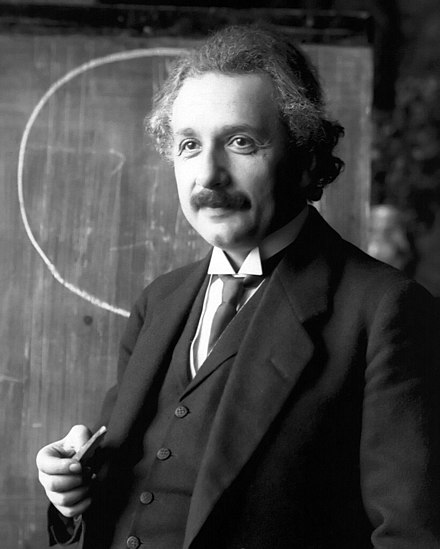
\includegraphics[width=8cm, height=8cm, keepaspectratio=true]{./content/Content-ulgr/autor1}
\end{center}

%% -- Die Referenzen werden am Ende des jeweiligen Beitrags ausgegeben
%% -- 
\smallskip
\begin{refsection}
\dictum[\href{https://de.wikipedia.org/wiki/Winston_Churchill}{Winston Churchill}]{Ein kluger Mann macht nicht alle Fehler selbst. Er gibt auch anderen eine Chance.}
%%
\begin{quote}
Dies ist eine Testdatei und kann als Beispiel dienen.
Für die eigene Eingabe des Beitrags kann man diesen Inhalt löschen oder auch nutzen.

Dies ist ein Typoblindtext. 
An ihm kann man sehen, ob alle Buchstaben da sind und wie sie aussehen. 
Manchmal benutzt man Worte wie Hamburgefonts, Rafgenduks oder Handgloves, um Schriften zu testen. 
Manchmal Sätze, die alle Buchstaben des Alphabets enthalten -- man nennt diese Sätze \enquote{Pangrams}. 
Sehr bekannt ist dieser: {\selectlanguage{english} The quick brown fox jumps over the lazy old dog} (siehe hierzu den \href{https://www.blindtextgenerator.de}{Blindtextgenerator›}
\end{quote}
%% 
\section*{Einige Definitionen}
\subsection*{Mathematische Umgebungen}
Definiert sind
\begin{verbatim}
\begin{theorem} \ldots \end{theorem}
\begin{thm} \ldots \end{thm}
\begin{proposition} \ldots \end{proposition}
\begin{prop} \ldots \end{prop}
\begin{corollary} \ldots \end{corollary}
\begin{cor} \ldots \end{cor}
\end{verbatim}
%%
\begin{theorem} 
	\ldots 
\end{theorem}
%%
\begin{proposition} 
	\ldots 
\end{proposition}
%%
\begin{corollary} 
	\ldots 
\end{corollary}
%%
\subsection*{Mathematische Symbole}
%
\begin{verbatim}
\N, \Z, \Q, \R, \C
\end{verbatim}
%%
$ \N $, $ \Z $, $ \Q $, $ \R $, $ \C $.
%%
\subsection*{Aufzählungen}
%%
Dazu wird das Paket \texttt{enumitem} von \textcite{enumitem} verwendet.
Möglichkeiten:
%%
\begin{verbatim}
\begin{enumerate}
 	\item
	Item
\end{enumerate}
\end{verbatim} 
%%
gibt
%%
\begin{enumerate}
 	\item
	Item
\end{enumerate}
%%
oder
%%
\begin{verbatim}
\begin{enumerate}[(a)]
 	\item
\end{enumerate}
\end{verbatim}
%%
gibt
%%
\begin{enumerate}[(a)]
 	\item
	Item
\end{enumerate}
%%
Also durch \verb|\begin{enumerate}[(i)]| entsprechend
%%
\begin{enumerate}[(i)]
 	\item
	Item
\end{enumerate}
%%
Mit der $^{*}$-Variante dann auch im Fließtext, etwa
%%
\begin{enumerate*}[(a)]
 	\item
	Item1
	\item
	Item2; 
\end{enumerate*}
%%
einfach ausprobieren.
%%
\subsection*{Texteingabe}
%%
Mittels \verb|\dh| bekommt man korrekt \dh und nicht d.h. -- gilt für \ua auch.
Weiteres ist im \texttt{ReadMe.md} beschrieben. 
Und die richtigen \enquote{Gänsefüßchen} bekommt man mit \verb|\enquote{Gänsefüßchen}|.

Aber auch nicht vergessen:
%%
\begin{itemize}[nosep]
	\item
	Bindestrich - mittels \verb|-|, also \verb|Riemann-Integral| gibt Riemann-Integral
	\item
	Gedankenstrich -- mittels \verb|--|, also \verb|Seite 100--120| gibt Seite 100--120
	\item
	Minuszeichen $ -1 $ mittels \verb|$ -1 $|.
\end{itemize}
%%


%% -- Begin des eigenen Artikels; diesen \blindtext kann man löschen (Test)
%% --
\section*{Erster Hauptabschnitt}		%% 
\subsection*{Erster Unterabschnitt}		%% 
\subsubsection{}	 \blindtext				%% Nur Nummerierung; eventuell sinnvoll, sonst weglassen
\subsubsection{}	 \blindtext	
%%				
\subsection*{Zweiter Unterabschnitt}
\subsubsection{}	 \blindtext				%% Nur Nummerierung; eventuell sinnvoll, sonst weglassen
\subsubsection{}	 \blindtext[2]				%% Nur Nummerierung; eventuell sinnvoll, sonst weglassen
%% --
%% --
\section*{Zweiter Hauptabschnitt}		%% 
\subsection*{Erster Unterabschnitt}		%% 
\subsubsection{}	 \blindtext				%% Nur Nummerierung; eventuell sinnvoll, sonst weglassen
\subsubsection{}	 \blindtext	
%%
%% -- etc.
%% --

%% -- Literaturverzeichnis
%% --
\RaggedRight
\printbibliography
\end{refsection}

